\documentclass[output=paper]{LSP/langsci}  
\author{Víctor Lara Bermejo} 
\title{Spontaneous dubbing as a tool for eliciting linguistic data: the case of second person plural inflections in Andalusian Spanish}
\abstract{In this paper, I expound an innovative methodology employed to analyse the sociolinguistic evolution of a Peninsular Spanish phenomenon that has not been researched in depth until now. The use of a single pronoun to address a second person plural is attested in the southern Spanish region of Andalusia and it induces both 2nd person and 3rd person agreements, not following the standard pattern. These mismatches respond to several social factors analysed statistically. The most recent information available on this phenomenon dates back to the 1930’s, so the new data collected, through a methodology that lends itself to eliciting a high quantity of data (spontaneous dubbing), evidences the development of this phenomenon.
}

\maketitle 
\begin{document}

  
%  
% \\
% Víctor Lara Bermejo\\
% Universidad Autónoma de Madrid\\
% \\
 

\section{ Introduction}
Second person pronouns in most Peninsular Spanish varieties distinguish perfectly the number of addressees and the degree of politeness. There are four: two singular, two plural. For each grammatical number, there is one for formality and another one for informality (table 1).

All informal pronouns induce 2nd person inflections, whereas formal pronouns must agree in 3rd person (table 2). This is the standard usage in Peninsular Spanish or Spanish spoken in the Iberian Peninsula (Spain, except the Canary Islands).

\begin{table}
\begin{tabular}{lll} & Singular\par & Plural\par\\
\lsptoprule
 Formality\par & Usted\par & Ustedes\par\\
 Informality\par & Tú\par & Vosotros\par\\
\lspbottomrule
\end{tabular}
\label{tab:1}
\caption{Standard second person pronouns} 
\end{table}

\begin{table}
\begin{tabular}{lll} & Singular\par & Plural\par\\
\lsptoprule
 Formality\par & 3\textsuperscript{rd} person\par & 3\textsuperscript{rd} person\par\\
 Informality\par & 2\textsuperscript{nd} person\par & 2\textsuperscript{nd} person\par\\
\lspbottomrule
\end{tabular}
\label{tab:2}
\caption{Standard person agreement for second person pronouns} 
\end{table}

However, at some time in the past, the western part of Andalusia, the most southern region in Spain, eliminated the 2nd person plural pronoun (2pl), \textit{vosotros}, and levelled \textit{ustedes} for any 2pl, regardless of the formality or the informality. In spite of this feature, \citet{lara_uso_2010} proved that \textit{ustedes} can agree both in 2pl and 3rd person plural (3pl) with verbs, clitics or possessives (1 – 3). 

\ea
\gll Ustedes                     sois          hermanos\\
 You-nom.2pl.hon. be-2pl.pres.ind. siblings\\
\glt`You are siblings'
\z

\ea
\gll Ustedes             se     casáis     mañana\\
 You-nom.2pl.hon. refl.3pl. marry-2pl.pres.ind. tomorrow\\
\glt ‘You are getting married tomorrow’\\
\z

\ea
\gll A   ustedes        os          vi       ayer\\
 To you-nom.2pl.hon. 2pl.acc. see-1sg.pret.ind.   yesterday\\
\glt ‘I saw you yesterday’\\
\z

These agreement mismatches between the stressed pronoun and the other syntactic elements anchoring \textit{ustedes}, have not been explained or sufficiently investigated until now.

\begin{figure}
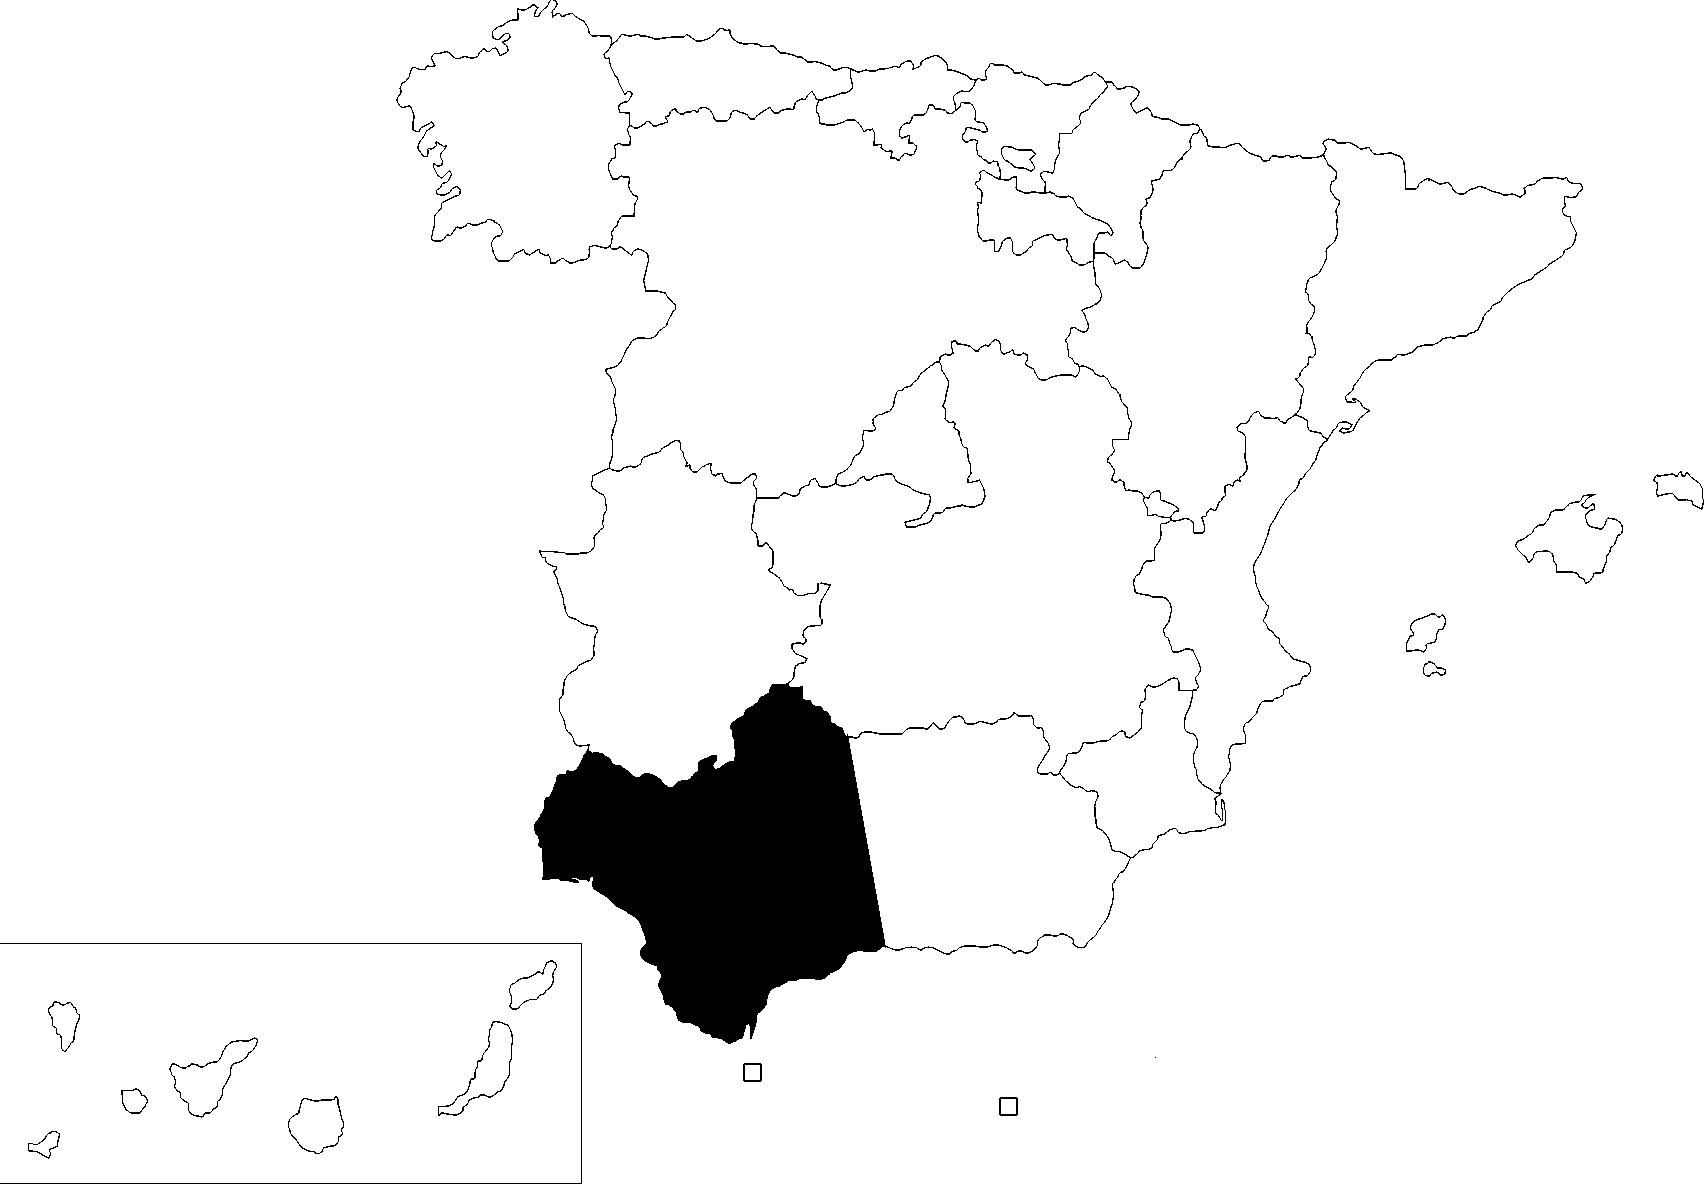
\includegraphics[width=\textwidth]{illustrations/lara_fig1}
\caption{Ustedes phenomenon inside Spain}
\end{figure}

\rmfamily
The literature about this phenomenon is found in works on historic grammars or monographs dealing with the Andalusian dialect \citep{mondejar_verbo_1974,lapesa_estudios_2000,cano_historia_2004,penny_variacion_2004,menendez_pidal_historia_2005}. These authors state that this vernacular feature is observed in the provinces of Córdoba, Málaga, Cádiz, Huelva and Seville (map 1). 

\rmfamily
They also state that it is stigmatised and it has always been considered as illiterate and rural. Furthermore, \textit{ustedes} always agrees in 2pl, unless the verb is tensed in past simple. In this case, the 3pl is preferred. Reflexive pronouns agree in 3pl, as well. All these linguists assure that the possessive has changed into the prepositional phrase de \textit{ustedes}, instead of the normative 3rd person \textit{su} or the 2pl \textit{vuestro} (table 3). The adoption of one specific person agreement does not take into account the politeness of the communicative situation.

\begin{table}
\resizebox{\textwidth}{!}{
\begin{tabular}{lp{.2\textwidth}p{.2\textwidth}p{.2\textwidth}p{.2\textwidth}p{.2\textwidth}p{.2\textwidth}} & Stressed pronoun & Verb & Past simple & Possessive & Reflexive pronoun & Object pronouns\\
\lsptoprule
 Formality & Ustedes & 2pl & 3pl & 3pl & 3pl & 2pl\\
 Informality  & Ustedes  & 2pl & 3pl & 3pl & 3pl & 2pl\\
\lspbottomrule
\end{tabular}
}
\label{tab:3}
\caption{Allocutives person agreements in Andalusia} 
\end{table}

As for many other phenomena, whenever a linguistic change arises, it does not do so in all the syntactic contexts it should \citep{labov_principles_1995,corbett_agreement_2006}. To illustrate, \textit{voseo} (the use of the medieval pronoun \textit{vós} to address one person in an informal context) first emerged in the stressed pronoun and its inflections spread gradually: first to the imperative, then to the present indicative, later to the present subjunctive but they are not attested yet in clitics and possessives \citep{fontanella_de_weinberg_oposicion_1979,abadia_de_quant_relacion_1992,bertolotti_synchronical_2003}. In the case of \textit{ustedes}, the 3pl was initially used in the stressed pronoun but it has not yet forced all its syntactic elements to be inflected in the 3pl, as will be shown hereinafter. It is reasonable to expect that the 3pl will spread gradually, until it is attested in all the \textit{ustedes} syntactic references.

As will be argued, some techniques employed in dialect data elicitation have not been useful to obtain 2pl inflections due to their low probability of emergence. The method I describe in this article represents a good pointer for the future study of dialects, thanks to the use of video dubbing and audiovisual stimuli. It can produce a large quantity of tokens to be analysed statistically, by avoiding any priming. In fact, this method has allowed to establish that the Andalusian dialect is beginning to comply with standard patterns. Thus, this paper is structured as follows: firstly, I describe previous methods for the collection of 2pl inflections in Andalusia; what has been found about the \textit{ustedes} linguistic behaviour and the shortcomings of these techniques. Later, I introduce my corpus and methodology and how they have compensated the lack of linguistic data from other sources. Then, I apply two statistical tests to the results of this new methodology. Finally, I focus on the development of the dialect phenomenon under study, in order to demonstrate the findings that my technique has led to.

\section{ALPI data}

The most recent information available on this phenomenon can be found in the Linguistic Atlas of the Iberian Peninsula (ALPI, by its Spanish acronym), uploaded on \citet{heap_atlas_2003}. This dialect atlas was conceived by Menéndez Pidal. However, it was a group of researchers who obtained the data by travelling throughout the Iberian Peninsula, with the aim of collecting the phonological, lexical and morpho-syntactic phenomena of all the Romance languages in the peninsula. Their interviews were carried out between the 1930’s and the 1950’s and these consisted of pre-established sentences and words that the informants had to repeat based on their vernacular variety \citep{sanchis_guarner_atlas_1962}. The lack of spontaneity could have tainted the informants’ responses. Although they could not rely on the electronic devices currently available, a great many of their linguistic findings are being validated in most recent research. 

Within the ALPI pre-established sentences, there are eleven with a reference to a 2pl. These provide data about the stressed pronoun, the reflexive pronoun, the accusative pronoun, as well as main verbs tensed in imperative and present indicative. A sentence with an embedded verb is also included. Thanks to this invaluable work, some information on the geographic diffusion pattern, the grammatical behaviour and the pragmatic incidence of this phenomenon could be disseminated.

\subsection{Geography}
In terms of geographic extension, this phenomenon is attested in West Andalusia, specifically in the provinces of Cádiz, Seville, Huelva, Córdoba (except the northern part) and Málaga (excepting the eastern part). Moreover, its diffusion pattern followed the wave model, as presented by \citet{chambers_dialectology_1980} or \citet{wolfram_dialectology_2003}. This model states that a specific linguistic phenomenon arises in a specific geographic point, called focus or epicentre, from which all the further innovations concerning the phenomenon also emerge in the first place. 

The hypothesis predicts that in an innovation in which three changes (C) have occurred, C1 arises in a specific point from which it is diffused toward its outlying area. When C1 has extended to the periphery, C2 appears in the same point where C1 had originated earlier. In an ulterior evolution, C2 reaches the outlying area of the focus, while C1 leaps to a more distant area, and, at the same time, an C3 arises in the focus.

If all this information is applied to the phenomenon under investigation, based on the ALPI data in map 2, several conclusions can be drawn.

\begin{figure}
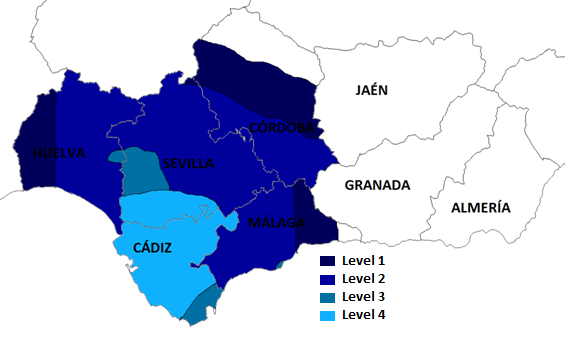
\includegraphics[width=\textwidth]{illustrations/lara_fig2}
 \caption{Andalusian geographic diffusion pattern \citep[85]{lara_ustedes_2012}.}
\end{figure}

The \textit{ustedes} phenomenon produced four changes, as map 2 shows. Level 1 is characterised by change 1; level 2 by changes 1 and 2; level 3, by changes 1, 2 and 3, and, finally, level 4 shows four changes. This spatial diffusion proves that the \textit{ustedes} phenomenon arose in Cádiz and southern Seville, as it is the region where all the changes initiate. The more proximate to this area, the more changes shared; the further away, the fewer changes shared, until the \textit{ustedes} phenomenon fades. 

\subsection{Grammar}
In terms of its grammatical behaviour, this phenomenon predicts the extension of the 3pl in all the syntactic elements anchoring \textit{ustedes}. Since \textit{ustedes} induces 3pl inflections, these must appear gradually, until they are settled in all the elements with reference to \textit{ustedes}. According to map 2, the extension of the 3pl follows an implicational hierarchy expressed in (4).

\begin{exe}
\ex Stressed pronoun {\textgreater} reflexive pronoun {\textgreater} accusative pronoun {\textgreater} embedded verb
\end{exe}

The continuum must be read as follows: the adoption of the 3pl in a specific grammatical element implies its emergence in the ones to the left. So, if the 3pl is attested in the accusative pronoun, it is also attested in the reflexive pronoun and, of course, in the stressed pronoun. This extension goes rightwards in the hierarchy.

Therefore, level 1 is characterised by the emergence of the 3pl in the stressed pronoun (5); level 2 is characterised by the extension of the 3pl in the reflexive pronouns (6); level 3, by the spread of the 3pl in the accusative pronoun (7) and, finally, level 4 shows that the 3pl is established in the embedded verb (8).

\ea
\gll Ustedes                   sois                      parientes del     alcalde\\
You-nom.2pl.hon. be-2pl.pres.ind. relatives of the mayor\\
\glt   ‘You are the mayor’s relatives’\\
\z

\ea
\gll Ustedes                    se            vais                      de viaje\\
You-nom.2pl.hon. refl.3pl. go-2pl.pres.ind. on trip\\
\glt   ‘You are going on a trip’\\
\z

\ea
\gll A  ustedes                    los          han                          engañado\\
To you-nom.2pl.hon. acc.3pl. have-3pl.pres.ind. lie-pcp.\\
\glt   ‘You have been deceived’\\
\z

\ea
\gll Haced           ustedes                  lo que      quieran\\ 
Do-2pl.imp. you-nom.2pl.hon. whatever want-3pl.pres.subj.\\
\glt   ‘Do whatever you want’\\
\z

\subsection{Pragmatics}
In terms of pragmatics, the informants’ grammatical agreement do not change based on the degree of politeness. According to the ALPI data, \textit{ustedes} is used both for formality and informality. The adoption of the 3pl or the maintenance of 2pl inflections are not affected by the type of addressees, as (9) and (10) show.

\ea
\gll ¿Adónde vais                      ustedes? (to children)\\
Where     go-2pl.pres.ind. you-nom.2pl.hon.\\
\glt   ‘Where are you going to’\\
\z

\ea
\gll Lo                     queréis                      para ustedes (to elderly people)\\
Acc.3sg.neut. want-2pl.pres.ind. for    you-nom.2pl.hon.\\
\glt   ‘You want it for yourselves’\\
\z

\section{Corpus and methodology}
In a typical sociolinguistic interview, the 2pl pronouns are the least likely to appear in a conversation. Thus, to analyse a phenomenon like the one studied here, it is not useful to collect data using this type of elicitation, since the informants tend to speak about themselves, about other people’s lives and they are also very likely to only address one interviewer although there may be two people posing questions. Pre-established sentences do not trigger a great many tokens, as ALPI demonstrates, since only one example for each pre-established sentence was recorded.

In order to compensate the shortcomings that arise in pre-established sentences and questionnaires, as well as the low probability of appearance of 2pl inflections through other more recent methods, I have devised another type of eliciting. It consists in having the informants dub a series of scenes compiled from the popular sitcom \textit{Friends} and the Spanish sitcom \textit{Aquí no hay quien viva} (‘It is impossible to live here’). Video stimuli have become quite an important tool for eliciting spontaneous and quantitative data in order to carry out an ulterior statistical analysis \citep{chelliah_handbook_2011,mallinson_data_2013,thieberger_oxford_2011,lara_tratamientos_2015}. The reason for choosing these two programmes lies in the dynamics that the scripts trigger since multiple dialogues, in which one or two characters have to address a group of people, naturally take place. In addition, these characters speak to addressees, with whom they either maintain a formal or informal social relationship: elderly people, bosses, flatmates, friends, neighbours, acquaintances, children, etc. It is, therefore, a great opportunity to analyse possible mismatches in the informants’ grammatical agreement, by taking also into account the formality of the given situation. The scenes are shown to informants, who are given a description with some lead sentences (cf.I), while they are watching the video. The scenes do not contain any sound and these provide a prompt, since the dubbing of the informants does not have to synchronise with the speech of the character they have to dub. Once they have understood the activity, they are asked to dub the character that is addressing the others, based on the previous oral synopsis and lead sentences. Each scene predicts the emergence of a specific syntactic element (verb, reflexive pronoun, object pronouns, and so on) thanks to these cue sentences. I have compiled several scenes so that each syntactic context can appear, in order to ensure the quantitative part of the corpus and its further analysis. No conditioning of the informants is possible, because the description of the scene is always carried out with references to third persons. Therefore, no 2pl is previously mentioned at all. All the fieldwork was carried out in 2012 and, thanks to this method, I have obtained approximately 4,500 occurrences from about 250 different informants. All of them were contacted through different educational institutions, depending on their level of literacy.

\subsection{Friends}
This sitcom was broadcast between the years 1994 and 2004, and it deals with the personal and social relationships that a group of close friends have with each other. Below, I describe some of the lead sentences that the informants had to reproduce in 2pl.

%%%
%%% roman enumerated list
%%%
\begin{enumerate}
\item [I] The main character is meeting some friends and they are all celebrating that she is getting married very soon. However, she is not as happy as she should be and starts pointing out to her friends all the things they can still do because they are single. (symmetrical communicative situation)\\
\\
\textbf{Syntactic context}: Present indicative and present subjunctive in embedded sentence.\\
\textbf{Lead sentence}: She says that they can do whatever they want. \\
\textbf{Expected sentence}: 

\ea
\gll {Podéis / pueden} {[ustedes / vosotros]} hacer {lo que} {[ustedes / vosotros]} {queráis / quieran}\\
{Can-\textsc{pres.ind.2pl/3pl}} \textsc{[nom.2pl.hon. / nom.2pl.]} do whatever \textsc{[nom.2pl.hon. / nom.2pl.]} want-\textsc{2pl / 3pl}\\
\glt {`You can do whatever you want.'}\\
\z

\textbf{Syntactic context}: Imperative, reflexive pronoun.\\
\textbf{Lead sentence}: She urges them not to get married.\\ 
\textbf{Expected sentence}:

\ea
\gll No   {os / se}               {caséis / casen}            {[ustedes / vosotras]}\\
Neg. {\textsc{refl.2pl / 3pl}} {get married-\textsc{pres.subj.2pl. / 3pl.}} {[nom.2pl.hon. / nom.2pl.]}\\
\glt {`Don’t get married.'}\\
\z

\item [II] The boss of one of the characters is in a meeting with the main character and a workmate. The boss asks them for their opinion on the new collection of clothing, which is about to be distributed on the market. (asymmetrical communicative situation)\\
\\
\textbf{Syntactic context}: Present indicative, interrogative modality\\
\textbf{Lead sentence}: She asks them for their opinion about the new collection.\\
\textbf{Expected sentence}:

\ea
\gll
{¿Qué}    {pensáis / piensan}           {[ustedes / vosotros]?}\\
What  {think-\textsc{pres.ind.2pl / 3pl}}    {\textsc{[nom.2pl.hon. / nom.2pl.]}?}\\
\glt {(‘What do you think about it?’)}\\
\z

\textbf{Syntactic context}: Conditional / reflexive pronouns / interrogative modality.\\
\textbf{Lead sentence}: She asks them whether they would wear the new collection.\\
\textbf{Expected sentence}:

\ea
\gll
{¿Os / se} {pondríais / pondrían}     {[ustedes / vosotros]}   la nueva colección?\\     
{\textsc{refl.2pl / 3pl}}  {wear-\textsc{cond. 2pl. / 3pl.}}  {\textsc{[nom.2pl.hon. / nom.2pl.]}} the new collection?\\
\glt {(`Would you wear this?')}\\
\z

\end{enumerate}

\subsection{Aquí no hay quien viva}
This sitcom was broadcast between the years 2003 and 2006, and it deals with the daily lives and relationships among neighbours of a residential building in the centre of Madrid. Some of the pre-established lead sentences are described below.

\begin{enumerate}
\item [III] A pair of friends wish to pretend to be a couple and they ask a friend of theirs how they can succeed in their pretence. Their friend answers by enumerating the conditions they have to fulfill if they want others to believe them. (symmetrical situation)\\
\\
\textbf{Syntactic context}: Future or present indicative.\\
\textbf{Lead sentence}: He says that they have to know many things about each other.\\ 
\textbf{Expected sentence}:

\ea
\gll
{Tendréis / tendrán / tenéis / tienen}                  {[ustedes / vosotros]} que saber cosas {el uno del otro}\\
{Have-\textsc{fut.ind.2pl / 3pl /-pres.ind.2pl / 3pl}}   {\textsc{[nom.2pl.hon. / nom.2pl.]}} to know things {about each other}\\
\glt (`You have to know things about each other.')\\
\z
 
\item [IV] The director of a bank office informs a couple that the bank cannot grant them a loan. (asymmetrical communicative situation)\\
\\
\textbf{Syntactic context}: Dative pronoun\\
\textbf{Lead sentence}: He tells them that the bank cannot grant them a loan. \\
\textbf{Expected sentence}:

\ea
\gll
No    {os / les}            podemos                otorgar {[a ustedes / vosotros]} el préstamo.\\
{\textsc{Neg.}} {\textsc{dat.2pl / 3pl}} {can-\textsc{pres.ind.1pl.}}  {grant}    {\textsc{[obl.2pl.hon. / nom.2pl.]}} the loan\\
\glt (`We cannot grant you the loan.')
\z

\end{enumerate}

\section{Analysis}
All the data have been processed with a statistics programme (SPSS). Each occurrence is tagged based on its extra-linguistic and linguistic factors. To illustrate, every example provides information about the social factors of the informant that has produced it: gender, age, educational level, locality, province, ALPI zone (cf. map 2) and size of the population of the locality. Moreover, the linguistic factors that have been established to analyse the agreement are the stressed pronoun, the reflexive pronoun, the accusative pronoun, the dative pronoun, the possessive, the verb tense, the verb mood, the modality, the type of embedded sentence and the communicative situation (formal or informal). Below, I reproduce the number of tokens and informants, on the basis of a number of their social features.

\begin{table}
\begin{tabular}{lll} & INFORMANTS & OCCURRENCES\\
\lsptoprule
MEN & 117 (48,3\%) & 2007 (44,6\%)\\
WOMEN & 125 (51,7\%) & 2484 (55,4\%)\\
TOTAL & 242 (100\%) & 4491 (100\%)\\
\lspbottomrule
\end{tabular}
\label{tab:4}
\caption{Informants and tokens (gender)}
\end{table}

\begin{table}
\begin{tabular}{lll} & INFORMANTS & OCCURRENCES\\
\lsptoprule
YOUNG & 94 (38,8\%) & 1956 (43,5\%)\\
WORKING POPULATION & 94 (38,8\%) & 1930 (42,9\%)\\
ELDERLY & 54 (22,4\%) & 605 (13,6\%)\\
TOTAL & 242 (100\%) & 4491 (100\%)\\
\lspbottomrule
\end{tabular}
\label{tab:5}
\caption{Informants and tokens (age)}
\end{table}

\begin{table}
\begin{tabular}{lll} & INFORMANTS & OCCURRENCES\\
\lsptoprule
HIGHER EDUCATION & 58 (24\%) & 1086 (24,1\%)\\
LOWER EDUCATION & 184 (76\%) & 3405 (75,9\%)\\
TOTAL & 242 (100\%) & 4491 (100\%)\\
\lspbottomrule
\end{tabular}
\label{tab:6}
\caption{Informants and tokens (educational level)}
\end{table}

\begin{table}
\begin{tabular}{lll} & INFORMANTS & OCCURRENCES\\
\lsptoprule
{}-5.000 INHAB. & 28 (11,5\%) & 489 (10,9\%)\\
5.000 – 10.000 INHAB. & 67 (27,7\%) & 1202 (26,7\%)\\
10.000 – 20.000 INHAB. & 63 (26\%) & 1149 (25,6\%)\\
20.000 – 100.000 INHAB. & 18 (7,5\%) & 252 (5,6\%)\\
100.000 – 500.000 INHAB. & 41 (17\%) & 872 (19,4\%)\\
+500.000 INHAB. & 25 (10,3\%) & 527 (17,8\%)\\
TOTAL & 242 (100\%) & 4491 (100\%)\\
\lspbottomrule
\end{tabular}
\label{tab:7}
\caption{Informants and tokens (size of the population)}
\end{table}

I have applied two statistical tests: the Pearson’s chi squared test and a logistic regression. The former gives the real significance of an independent variable (ie: gender, age, etc.) and the latter orders the degree of affectedness of each significant variable. Below, I detail the results of this methodology, applied to the \textit{ustedes} phenomenon, taking into account three parameters: the geographical factor, the sociolinguistic factor and the linguistic factor.

\subsection{Geographic factor}
I have classified the occurrences of the phenomenon, based on its percentage. Hence, map 3 shows to what extent the \textit{ustedes} phenomenon is attested in speakers. This map is based on the ALPI zones (cf. map 2). As map 3 shows, in the area marked A, the informants manifest the \textit{ustedes} misagreement feature over 66\% of the time. In area B, the informants are characterised by an intermediate degree of dialectalism (33\% - 66\%). Finally, part C represents the area in which the \textit{ustedes} phenomenon appears less than 33\% of the time. 

\begin{figure}
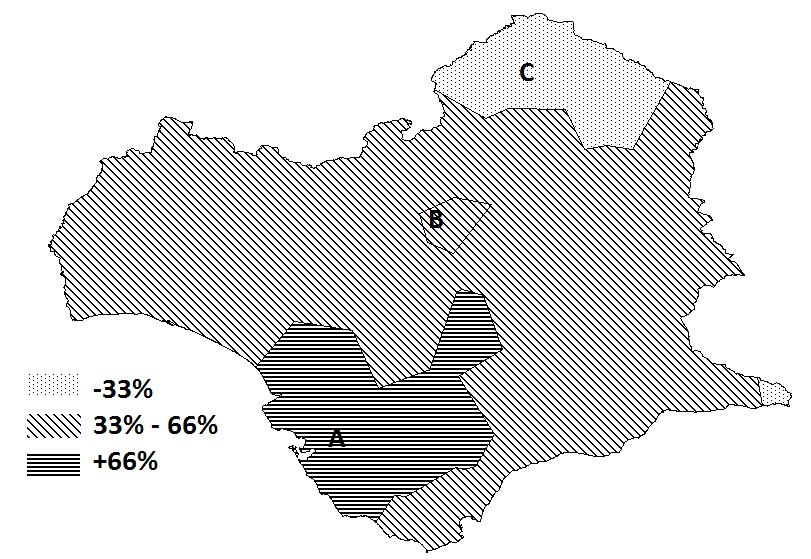
\includegraphics[width=\textwidth]{illustrations/lara_fig3}
\label{fig:3}
\caption{Percentage of use of ustedes, based on the ALPI zones}
\end{figure}

Where Cádiz and Seville are the districts with a higher proportion of maintenance of the phenomenon, Córdoba and Málaga behave in the opposite fashion, while Huelva takes up the middle ground. The \textit{ustedes} phenomenon has not extended further than it had almost one hundred years earlier. Indeed, in some parts where ALPI had recorded this phenomenon I have not found any instances. It can be deduced that it is probable that the \textit{ustedes} phenomenon has decreased in geographical terms. This regression has taken place in northern Córdoba. Nevertheless, the conclusion is that the further away from the focus, the likelier to imitate the standard usage: the closer to the ALPI focus or epicentre (Cádiz and southern Seville), the greater the likelihood that this vernacular phenomenon is maintained. 

If the percentages are divided on the basis of the size of the population of the locality surveyed, the results are quite different, as map 4 shows.

\begin{figure}
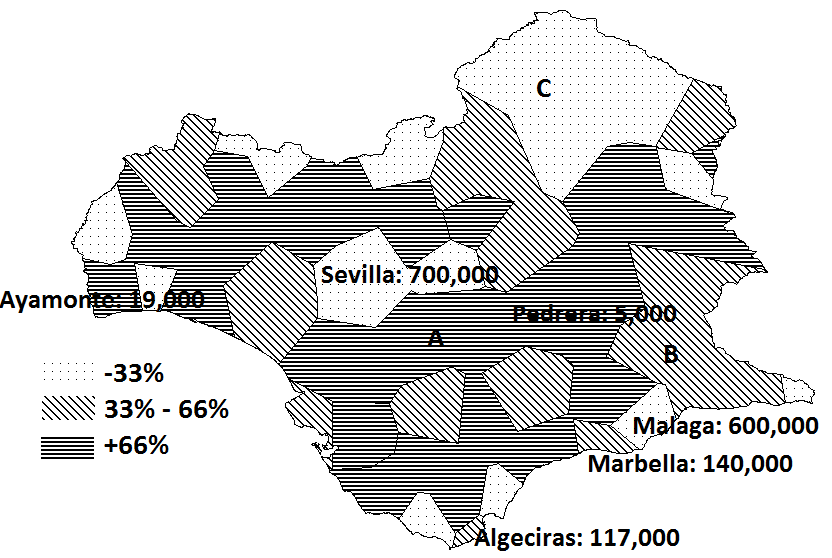
\includegraphics[width=\textwidth]{illustrations/lara_fig4}
\label{fig:4}
\caption{Percentage of use of ustedes, based on the locality surveyed}
\end{figure}
  
This map reveals that the use of the vernacular feature is greater when the municipality has fewer inhabitants. Despite the high variation, there seems to be a clear distinction between large cities, such as Seville and Málaga, and towns (Marbella and Algeciras) and villages (Ayamonte and Pedrera). The first try to adopt the standard usage, while the remaining two are more conservative and prefer to maintain the vernacular phenomenon. In all the statistical results related to population, the smaller the town is, the likelier they maintain the vernacular phenomenon. This may lead to the conclusion that another kind of spatial diffusion of the standard use is taking place in detriment of the dialect feature: the gravity model. This pattern predicts that a given linguistic phenomenon will be extended depending on the population density of two points \citep{wolfram_dialectology_2003}.

\subsection{Sociolinguistic factor}
The Pearson’s chi squared test for the \textit{ustedes} phenomenon has proved that the use of the vernacular or the standard pattern depends on the informants’ age, educational background and the municipality in which they live. In addition, the logistic regression shows that the first factor that conditions the use of the vernacular feature is the educational background, followed by the age and, then, the size of the population of the locality. This implies that the higher the educational background of the informants, the lower their tendency toward the vernacular. As a sample of this, I reproduce the table and figure taken from the statistical analysis.

\begin{table}
\begin{tabular}{ll|cc|l}
\lsptoprule

& & \multicolumn{2}{c|}{Educational level} & Total\\
& & Low & High & \\

SUBJECT U / V & U & 116 & 16 & 132\\

& U / V & 53 & 44 & 97\\

Total & & 169 & 60 & 229\\

\lspbottomrule
\end{tabular}
\caption{Occurrences in informants, based on their educational level}
\label{tab:8}
\end{table} 

%%%
%%% the right columns are empty --- correct?
%%%
\begin{table}
\begin{tabular}{llllll}
\lsptoprule
\multicolumn{6}{c}{\bfseries Pearson’s chi squared}\\
\midrule
& Value & gl & 
\begin{minipage}[t]{0.15\textwidth}Sig. asintotical (bilateral)\end{minipage} & 
\begin{minipage}[t]{0.15\textwidth}Sig. exact (bilateral)\end{minipage} & 
\begin{minipage}[t]{0.15\textwidth}Sig. exact (unilateral)\end{minipage} \\
\midrule
\begin{minipage}[t]{0.15\textwidth}Chi-squared Pearson\end{minipage} & 31,949\textsuperscript{a} & 1 & ,000 &  & \\
\begin{minipage}[t]{0.15\textwidth}Valid cases\end{minipage} & 229 &  &  &  & \\
\lspbottomrule
\end{tabular}
\label{tab:9}
\caption{Pearson’s chi squared test applied to educational level} 
\end{table}

\begin{figure}
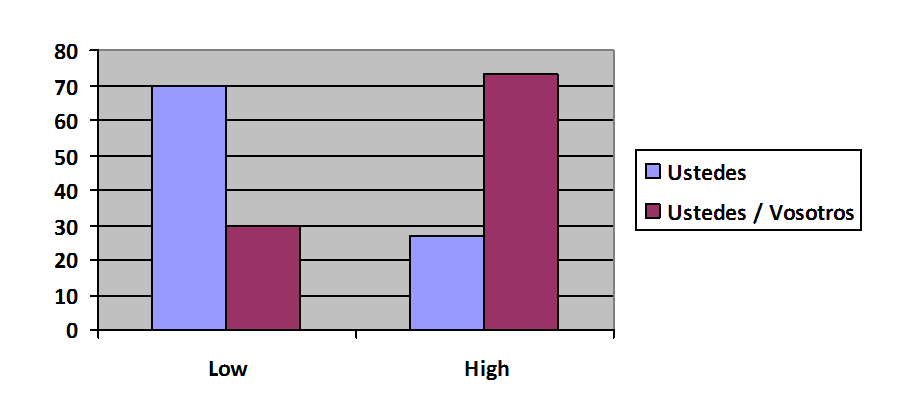
\includegraphics[width=\textwidth]{illustrations/lara_fig5}
\label{fig:5}
\caption{Percentage of use of ustedes, based on the educational level}
\end{figure}

Tables 8 and 9 show that the educational level produces a high significance rate. Only 53 speakers out of the 169 informants with a low educational level distinguish between \textit{vosotros} and \textit{ustedes}, while 44 people (out of 60) with a high educational background do so. This means that nearly 80\% of informants with a higher education prefer to follow the standard pattern (to distinguish \textit{ustedes} and \textit{vosotros}) while hardly 30\% of those with a lower education choose this model. Furthermore, if the variable age is taken into account (figure 2), other conclusions can be drawn.

\begin{figure}
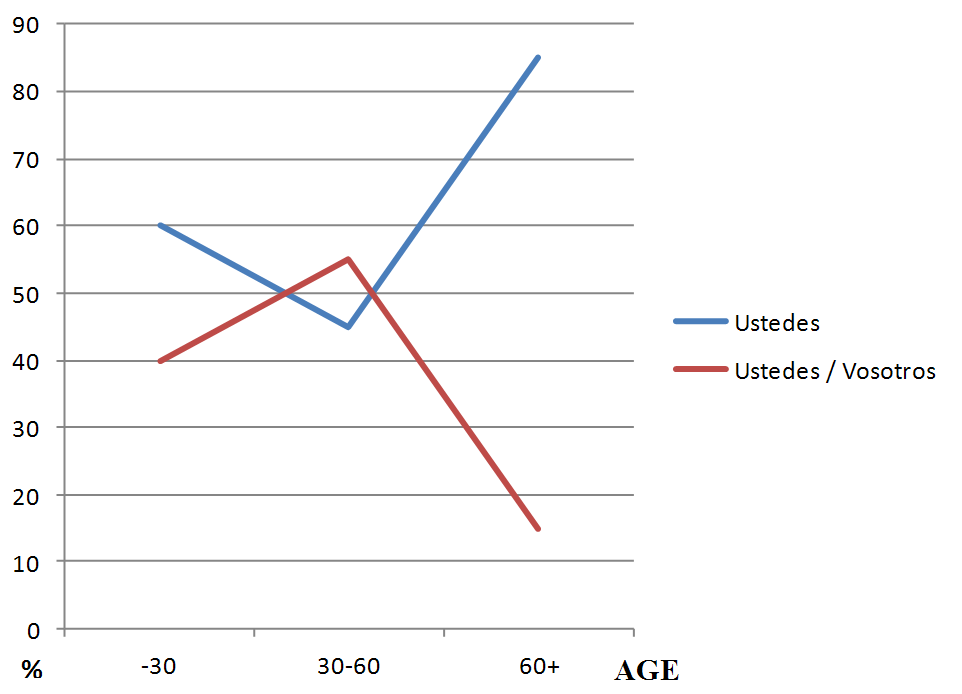
\includegraphics[width=\textwidth]{illustrations/lara_fig6}
\label{fig:6}
\caption{Percentage of use of ustedes, based on the informants' age}
\end{figure}

\figref{fig:6} clearly shows that the informants that have reached working age choose the prestigious norm, as they favour the standard in a higher proportion. They are closely followed by speakers younger than 30. At the opposite end, the elderly informants have a low sensitivity toward the standard form. According to \citet{chambers_dialectology_1980}, a situation like the one described is due to the fact that young people are less pressured by the standard and their linguistic behaviour responds to the uses their social networks positively value. The elderly also follow this pattern, since they do not belong to the labour environment, which, on the other hand, is crucial to the working-age population. In fact, these assume a different behaviour than the rest of the age groups. Their integration into the work force leads them to adopt the prestige form in order to succeed in their careers \citep{macaulay_language_1977,bourdieu_mercado_1978,seara_variacao_2000}. According to \citet{chambers_dialectology_1980}, a result like this is not a solid proof of a change in progress. Moreover, this result predicts that the new speakers will behave the same way, depending on the age group to which they belong. So, the new young people will imitate this behaviour because they are less pressured by the standard; once they are of working age, they will try to adopt the prestige and, when that phase is over, they will be freer to readopt their most vernacular features.

\subsection{Linguistic extension}
As mentioned at the beginning of this article, the 3pl was not attested in all the syntactic elements anchoring \textit{ustedes} and the extension of the 3pl was expected to occur gradually in syntax. The results obtained through my methodology have demonstrated that the syntactic elements agreeing with \textit{ustedes} adopt the 3pl as follows:

\begin{exe}
\ex Stressed pronoun {\textgreater} reflexive pronoun {\textgreater} verb {\textgreater} accusative pronoun {\textgreater} dative pronoun {\textgreater}
\end{exe}

The hierarchy must be read this way: if the 3pl appears in the accusative pronoun, it must also arise in the verb, the reflexive pronoun and the stressed pronoun. Only when the 3pl is set in one element, does it pass to the other, always rightwards. Unlike ALPI data, this methodology has allowed the elicitation of all the syntactic elements referring to \textit{ustedes}. Contrary to the statements made by \citet{mondejar_verbo_1974}, \citet{lapesa_estudios_2000}, \citet{cano_historia_2004}, \citet{penny_variacion_2004} or \citet{menendez_pidal_historia_2005}, possessives hardly agree in 3pl –indeed, they are the elements the least likely to adopt it. Object pronouns behave more independently than the reflexive pronouns. In fact, dative pronouns are quite reluctant to agree in 3pl (table 10). 

\begin{table}
\resizebox{\textwidth}{!}{
\begin{tabular}{lp{0.15\textwidth}p{0.15\textwidth}p{0.15\textwidth}p{0.15\textwidth}p{0.15\textwidth}p{0.15\textwidth}} 
& Stressed pronoun & Reflexive pronoun & Verbs & Accusative pronoun & Dative pronoun & Possessives\\
\lsptoprule
 Stage 1 & 3pl & 2pl & 2pl & 2pl & 2pl & 2pl\\
 Stage 2 & 3pl & 3pl & 2pl & 2pl & 2pl & 2pl\\
 Stage 3 & 3pl & 3pl & 3pl & 2pl & 2pl & 2pl\\
 Stage 4 & 3pl & 3pl & 3pl & 3pl & 2pl & 2pl\\
 Stage 5 & 3pl & 3pl & 3pl & 3pl & 3pl & 2pl\\
 Stage 6 & 3pl & 3pl & 3pl & 3pl & 3pl & 3pl\\
\lspbottomrule
\end{tabular}
}
\label{tab:10}
\caption{Extension of the innovative 3pl in the ustedes phenomenon} 
\end{table}

As explained above, the extension of innovations follows implicational hierarchies. \citet{blake_case_2004} states that in many languages, any innovation usually obeys the continuum reproduced in (12).

\begin{exe}
\ex Nominative {\textgreater} accusative {\textgreater} dative {\textgreater} ablative {\textgreater} genitive
\end{exe}

This means that if a language has a mark for any syntactic status, it also has one for those on the left. If this hierarchy is applied to some linguistic phenomena, Blake states that in some languages, relativisation follows this continuum. If one language can relativise the direct object, it can also do so to its subject. The same applies to passive sentences. Spanish can have a passive with direct objects in actives, but not with indirect objects. English, nonetheless, can even have a passive with an indirect object, so it can also do so with accusatives. In the \textit{ustedes} phenomenon, this hierarchy is completely fulfilled, as the 3pl emerges on the nominative and shifts over to the next syntactic context until the 3pl is established in the whole continuum.

\section{Conclusions}
To summarise, the innovative methodology designed for obtaining quantitative and qualitative data about the \textit{ustedes} phenomenon has been a success, in comparison to other traditional methods, unable to collect instances of 2pl inflections. Therefore, thanks to my fieldwork, it is possible to know that nowadays, some Andalusian speakers are characterised by a high rate of alternation between the standard and the vernacular feature, with respect to the 2pl pronouns system. On the one hand, there is a dramatic tendency toward the prestige and standard usage, and this behaviour is led, above all, by middle-aged speakers with a high educational background, and who live in large urban environments. This new change seems to be spreading hierarchically, unlike the wave diffusion pattern attested last century. The standard pressure is firstly observed in the populous cities of Seville and Málaga. Therefore, the smaller towns are likelier to maintain the vernacular phenomenon.

On the other hand, rural, elderly and not very educated speakers maintain the vernacular in their linguistic behaviour. In this case, the 3pl extends linguistically across an implicational continuum. The stressed pronoun is the one where it is first attested, then it passes onto the reflexive pronoun, followed by the verb and it extends to the accusative and the dative pronouns, in this order. Finally, possessives are the syntactic contexts with the least probability to be inflected in 3pl.

This method for eliciting linguistic data is an important tool in order to obtain a large amount of tokens for their ulterior statistical analysis, without priming. Furthermore, having informants carry out an activity that may be perceived as leisurely can lead to more spontaneous data. Audiovisual prompting is a productive method for the recollection of dialect data and the method I have introduced here will certainly be useful to others in the future.

\printbibliography[heading=subbibliography,notkeyword=this]
\end{document}
